\documentclass[11pt]{article}
\usepackage{graphicx}
\graphicspath{ {.} }
\title{Project 1 - Markovian Queue Implementation}
\author{Harshavardhan Nalajala}
\date{October 23 2017}
\begin{document}
\maketitle
 \tableofcontents
 
 \section{Description}
 Purpose of this project is to implement and run simulation of finite population, finite capacity, finite servers continuous time markov process system.
 Service times of servers are exponential. Arrival rate is poisson with inter arrival times being exponential. 
 Assumptions: 
 \begin{itemize}
 \item Service times of all servers are equal and there is no priority for a request arriving.
 \item A terminal is blocked when there is a request corresponding to the terminal either being processed or in queue.
 \end{itemize}
 \section{Implementation}
 Following is the implementation detail with L(no. of terminals), K(capacity of the system including queue size and requests in service), m(no. of servers), mu(service time of all servers)
 \begin{itemize}
 \item For lambda ranging between 0.01*mu*m to 1*mu*m
 
 \begin{itemize}
 \item Generate L requests with rate lambda and add them to min heap.
 \item while number of departures is not total(100000 for testing purposes)
 
 \begin{itemize}
 \item get the top event from min heap i.e. min element in heap (ordered by time).
 \item If the request in event is ARRIVAL:
 
 \begin{itemize}
 \item If system size is K, drop the request and generate arrival event for the corresponding terminal, and add this new event to heap.
 \item If system size is less than K, and greater than m, add the request to queue (requests are ordered by time of arrival).
 \item If system size is less than m, generate departure event and add to min heap.
 \end{itemize}
 
 \item If the request in event is DEPARTURE:
 
 \begin{itemize}
 \item If there are requests in queue, generate departure event to the first request in queue, and add to min heap.
 \item If total departure is less than TOTAL, generate arrival event for the corresponding terminal and add to min heap.
 \item If total departure is TOTAL, exit.
 \end{itemize}
 
 \end{itemize}
 \end{itemize}
 \end{itemize}
 
 \section{Data Structures }
 \begin{itemize}
 \item Min Heap to store the requests ordered by time. Event that occurs in the most near future is stored at the root of the heap. Max heap size is dependent on the requests generated.
 In the current project, heap size is dependent on L(no. of terminals) since each terminal cannot generate another request until current request from the terminal is processed by the system.
 \item Queue to store the requests that arrived at the system but servers are busy. Max queue size is order of K(Queue size).
 \end{itemize}
 
 \section{Performance Statistics}
 Statistics collection consists of
 \begin{itemize}
 \item Expected Number in the system: Each time arrival or departure happens, EN is given by (number in the system)*(current clock - prev event clock). Expected number is given by EN/totalClock at the end of simulation.
 \item Expected Time in the system: Each time departure happens, ET is given by (event departure time - event arrival time). Expected time is given by ET/totalDeparture at the end of simulation.
 \item blocking probability: no. of drops/total no. of arrival requests
 \item utilization: System busy time is calculated based on the number of requests in the system. If the no. of requests in the system is greater than or equal to no. of servers, system busy time is calculated as (no. of servers)*(current time - prev event time). If the no. of requests in the system is less than no. of servers, system busy time is calculated as (no. of requests in the system) * (current time - prev event time). Utilization is set to system busy time divided by (total servers * total clock) at the end of simulation.
 \end{itemize}
 \section{ReadMe}
 \begin{itemize}
 \item main.c contains the main simulation program (run\textunderscore simulation API).
 \item utils.c is used to store data structures and generate exponential random variables.
 \item utils.h contains the structures and API used by main.c and implemented in utils.c
 \item input.in contains the input to be given to the program. Following is the input style.
 \begin{itemize}
 \item no. of events to be generated for each run, 'run'
 \item no. of terminals, L
 \item queue size, K
 \item no. of servers, m
 \item service time of each server, 'mu'
 \end{itemize}
 \item plotter.py python script to generate the graphs of output obtained from simulation.
 \item avg\textunderscore output file contains the output as lambda, expected no., theoritical expected no., expected time, theoritical expected time, blocking probability, theoritical blocking probability, utilization of the system, theoritical utilization of the system.
 \item q\textunderscore simulator executable to be run.
 \item run\textunderscore script shell script file to build and run the simulation. Use following method to run the simulation.
 \begin{itemize}
 \item modify input.in as per above instructions
 \item ./run\textunderscore script.sh 
 \end{itemize}
 \end{itemize}
 \section{Dependencies}
 \begin{itemize}
 \item gcc compiler
 \item python3. For python2 or 2.7, run\textunderscore script needs to be modified to enable python2. 
 \end{itemize}
 \section{OUTPUTS}
 Performance measures obtained using simulation are compared to measures calculated theoritically in code. Following are the list of experiments done.
 
 \subsection{L10, K4, M2, U3}
 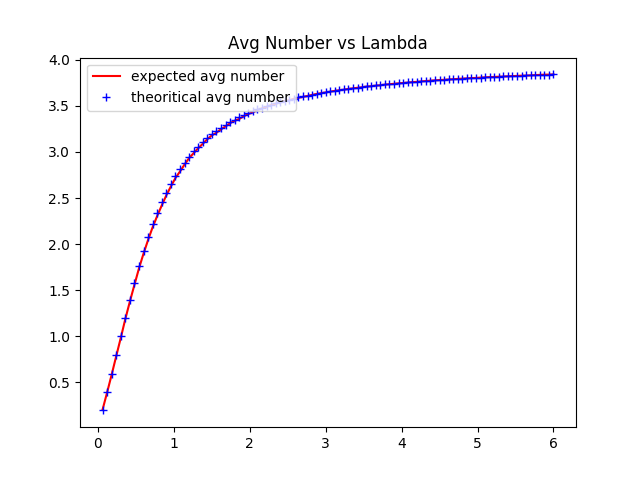
\includegraphics{ExpectedNumber_L10_K4_M2_U3}
  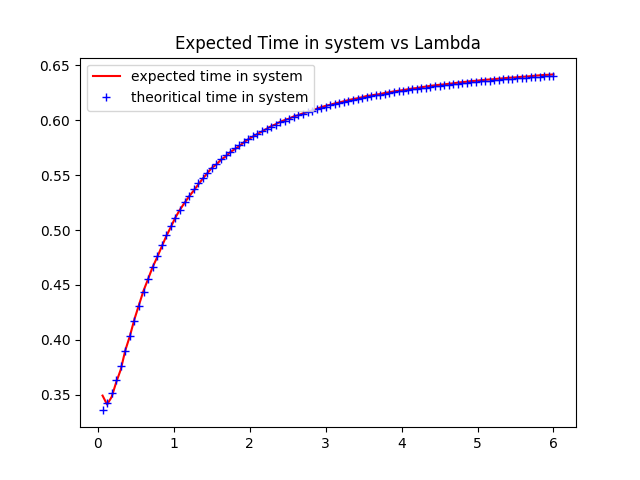
\includegraphics{ExpectedTime_L10_K4_M2_U3}
 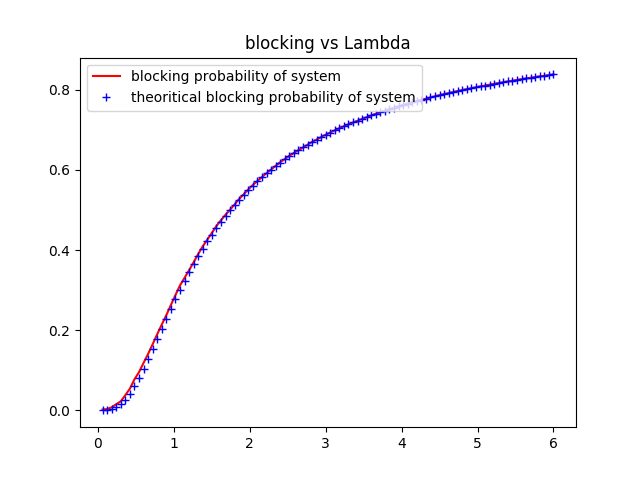
\includegraphics{BlockingProbability_L10_K4_M2_U3}
 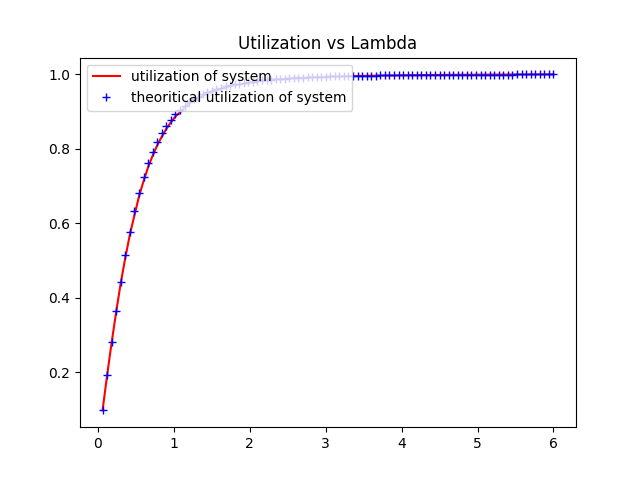
\includegraphics{Utilization_L10_K4_M2_U3}
 
 \subsection{L1, K4, M2, U3}
 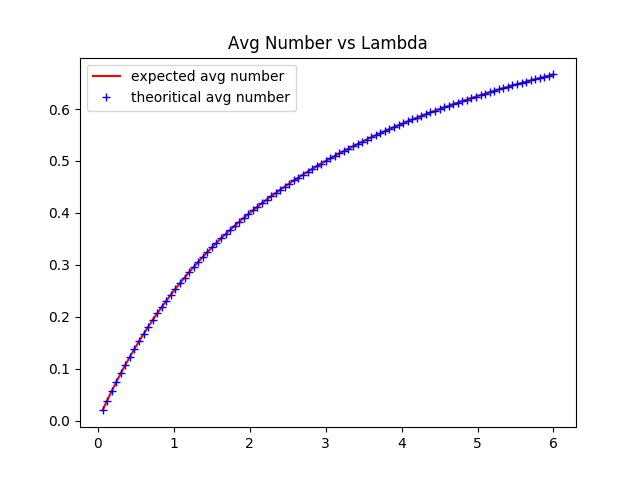
\includegraphics{ExpectedNumber_L1_K4_M2_U3}
  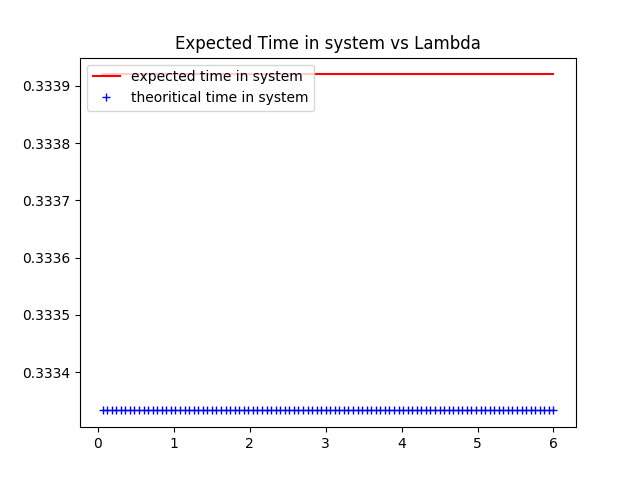
\includegraphics{ExpectedTime_L1_K4_M2_U3}
 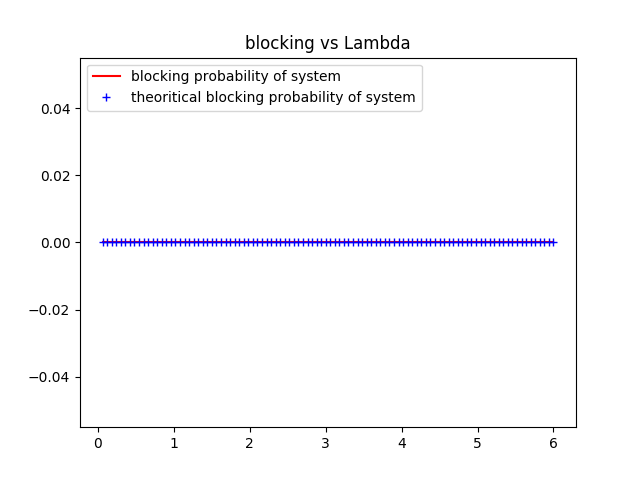
\includegraphics{BlockingProbability_L1_K4_M2_U3}
 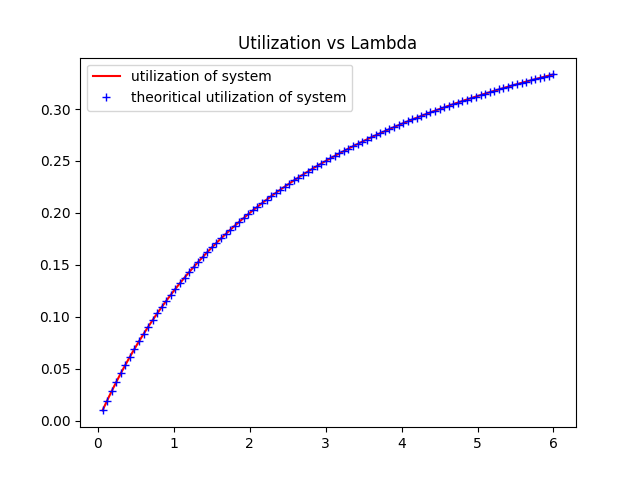
\includegraphics{Utilization_L1_K4_M2_U3}


 
  \subsection{L10, K4, M4, U3}
 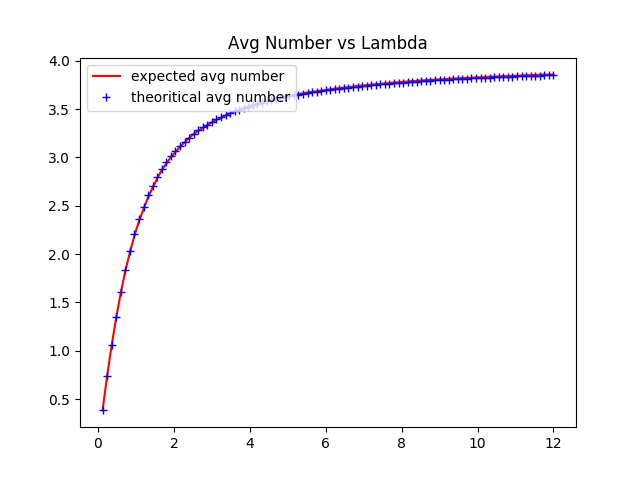
\includegraphics{ExpectedNumber_L10_K4_M4_U3}
  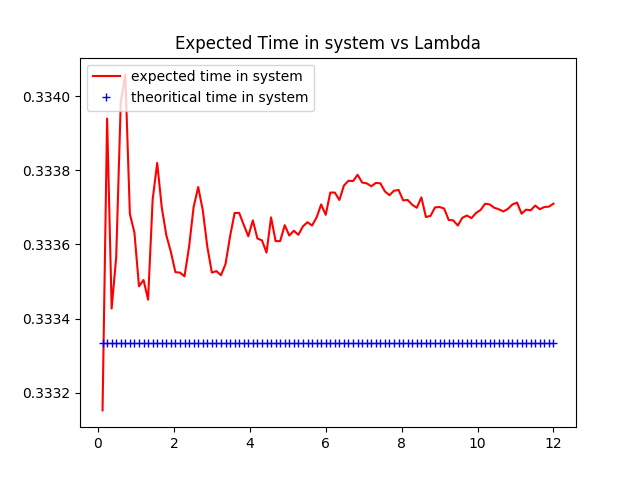
\includegraphics{ExpectedTime_L10_K4_M4_U3}
 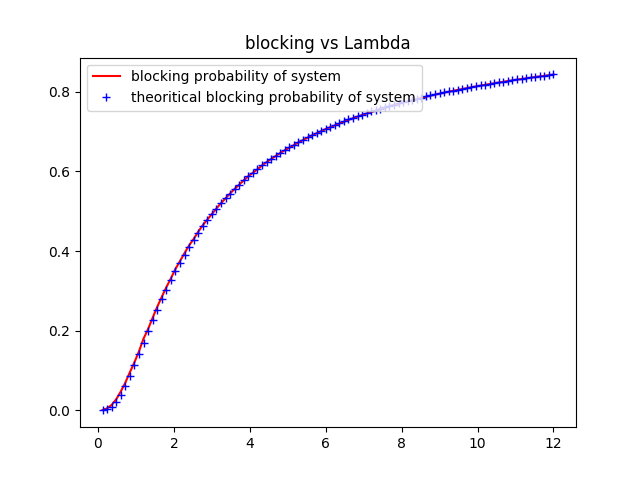
\includegraphics{BlockingProbability_L10_K4_M4_U3}
 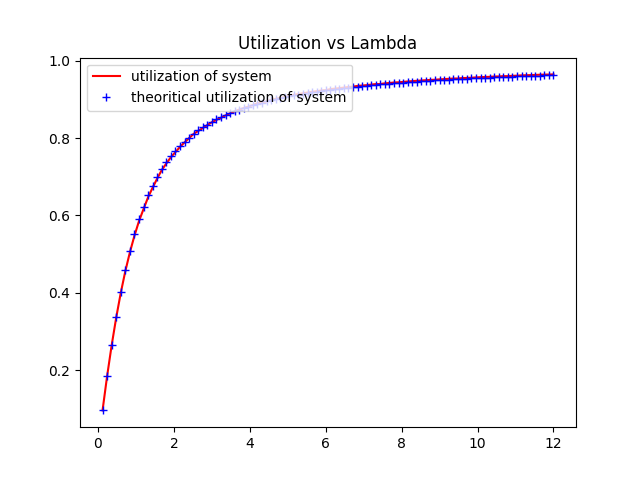
\includegraphics{Utilization_L10_K4_M4_U3}
 
  \subsection{L100, K30, M25, U3}
 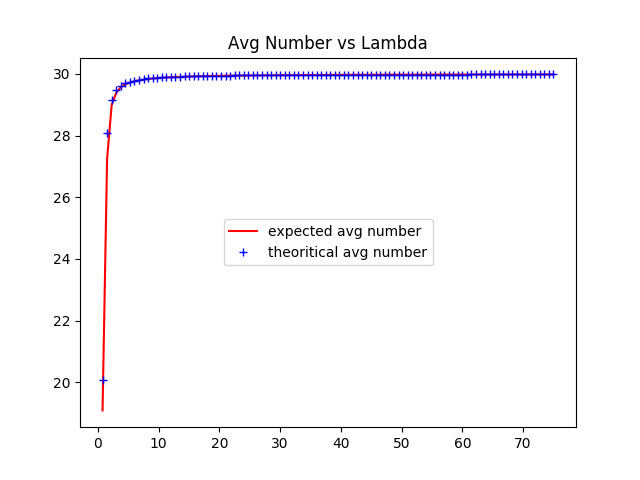
\includegraphics{ExpectedNumber_L100_K30_M25_U3}
  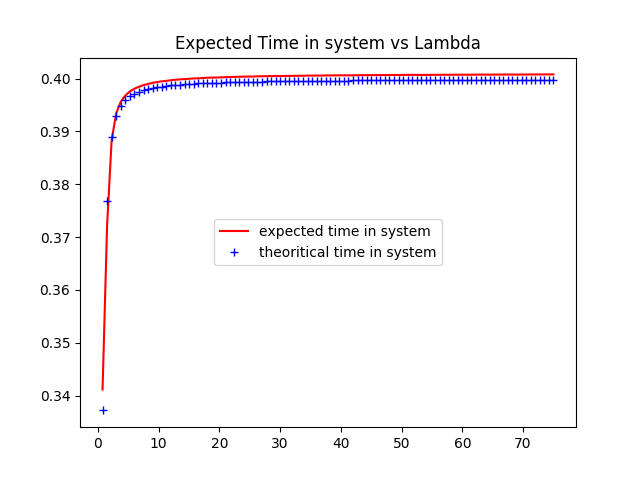
\includegraphics{ExpectedTime_L100_K30_M25_U3}
 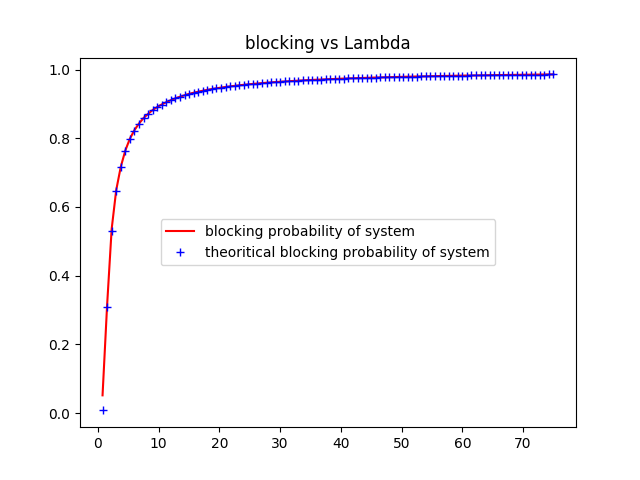
\includegraphics{BlockingProbability_L100_K30_M25_U3}
 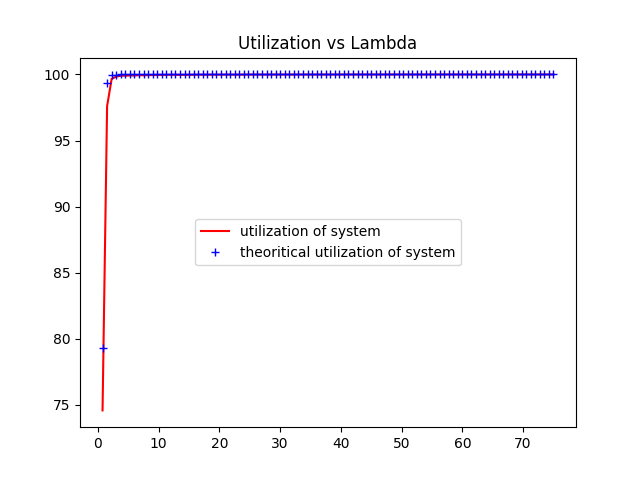
\includegraphics{Utilization_L100_K30_M25_U3}
 
  \subsection{L100, K75, M25, U10}
 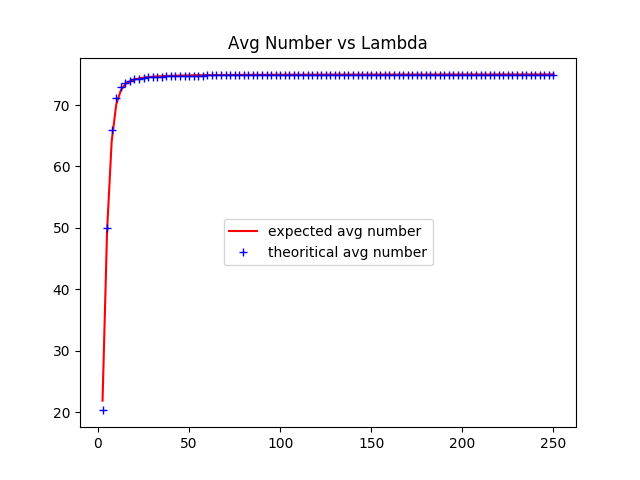
\includegraphics{ExpectedNumber_L100_K75_M25_U10}
  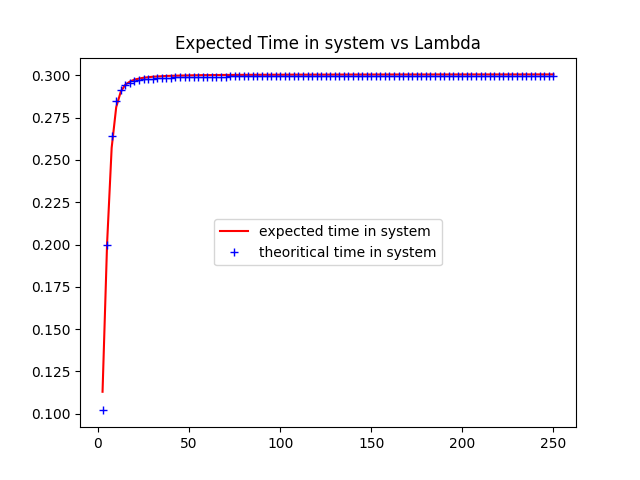
\includegraphics{ExpectedTime_L100_K75_M25_U10}
 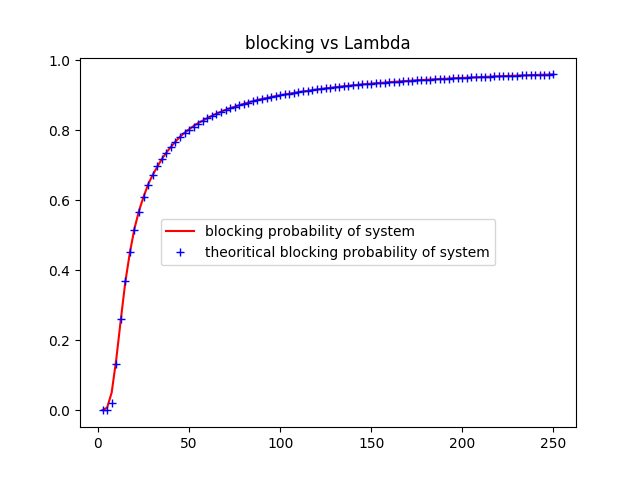
\includegraphics{BlockingProbability_L100_K75_M25_U10}
 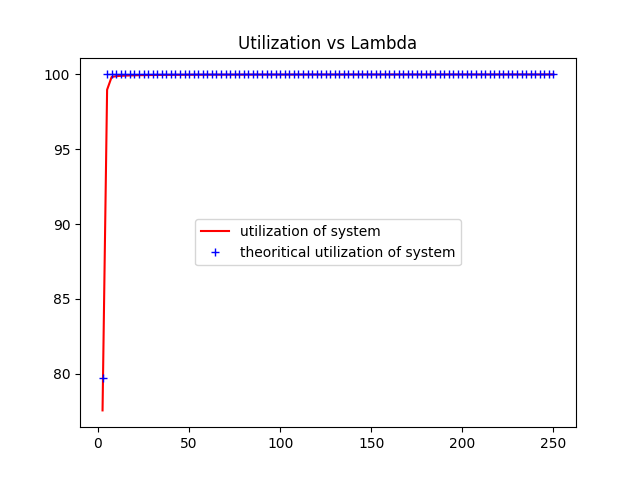
\includegraphics{Utilization_L100_K75_M25_U10}
 
 \subsection{L1000, K4, M2, U3}
 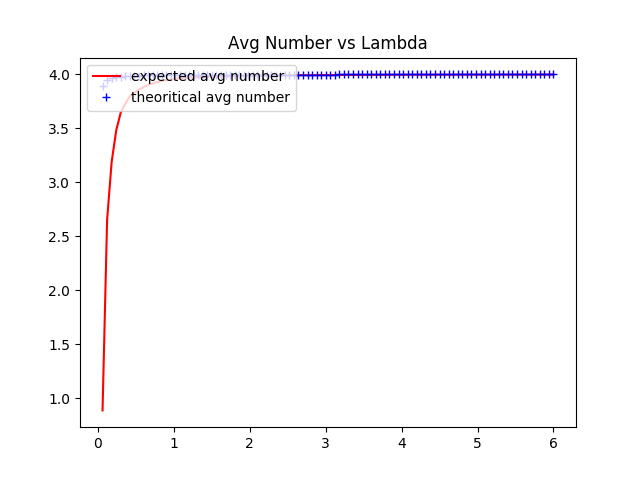
\includegraphics{ExpectedNumber_L1000_K4_M2_U3}
  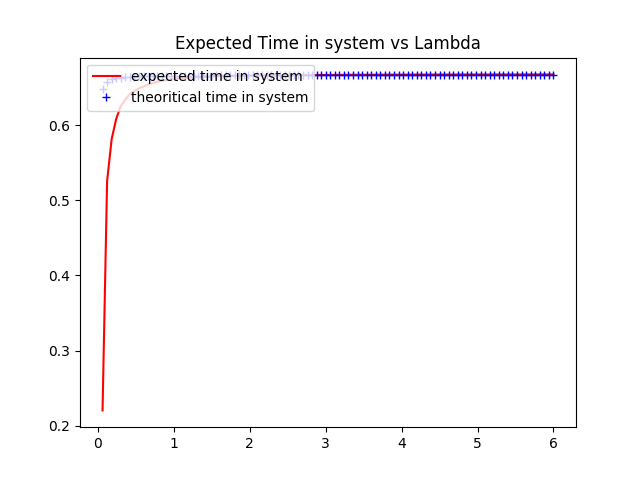
\includegraphics{ExpectedTime_L1000_K4_M2_U3}
 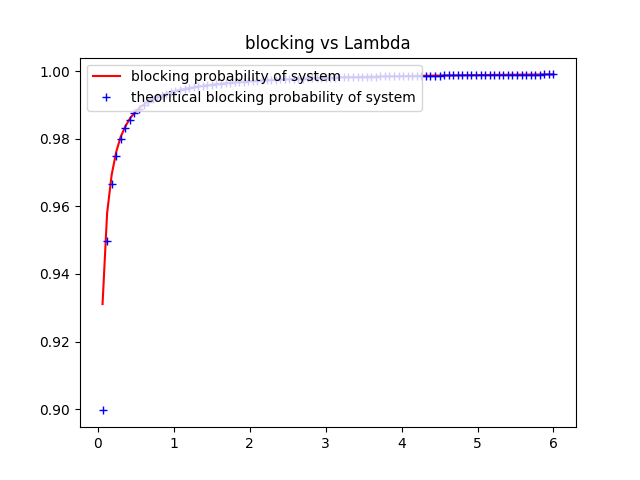
\includegraphics{BlockingProbability_L1000_K4_M2_U3}
 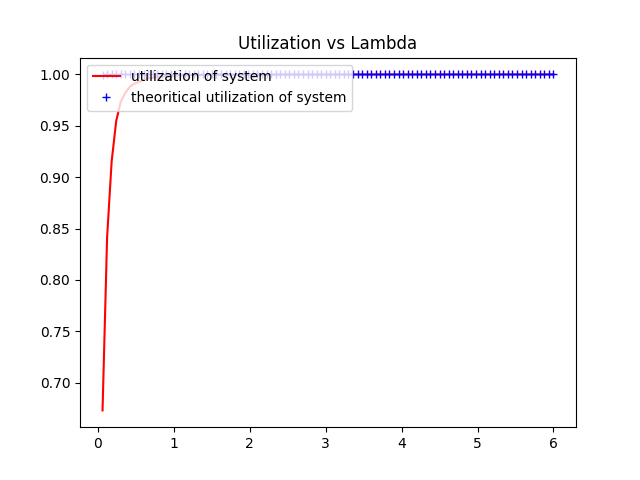
\includegraphics{Utilization_L1000_K4_M2_U3}
 

 
 \section{Limitations}
 Heap size is set to 10000 in utils.h. As long as number of events at any point of time is not more than 10000, simulator is fine. However we can modify the value and run the script again. Script builds the code and runs the simulation again.
\end{document}